%%%%%%%%%%%%%%%%%%%%%%%%%%%%%%%%%%%%%%%%%
% Tufte Essay
% LaTeX Template
% Version 2.0 (19/1/19)
%
% This template originates from:
% http://www.LaTeXTemplates.com
%
% Authors:
% The Tufte-LaTeX Developers (https://www.ctan.org/pkg/tufte-latex)
% Vel (vel@LaTeXTemplates.com)
%
% License:
% Apache License, version 2.0
%
%%%%%%%%%%%%%%%%%%%%%%%%%%%%%%%%%%%%%%%%%

%----------------------------------------------------------------------------------------
%	PACKAGES AND OTHER DOCUMENT CONFIGURATIONS
%----------------------------------------------------------------------------------------

\documentclass[a4paper]{tufte-handout} % Use A4 paper by default, remove 'a4paper' for US letter

\usepackage{graphicx} % Required for including images
\setkeys{Gin}{width=\linewidth, totalheight=\textheight, keepaspectratio} % Default images settings
%\graphicspath{{Figures/}{./}} % Specifies where to look for included images (trailing slash required)

\usepackage{amsmath, amsfonts, amssymb, amsthm} % For math equations, theorems, symbols, etc
%\usepackage{units} % Non-stacked fractions and better unit spacing
\usepackage{physics,siunitx}
\usepackage{cancel}

\usepackage{booktabs} % Required for better horizontal rules in tables
\usepackage{subfiles}

%----------------------------------------------------------------------------------------
%	TITLE SECTION
%----------------------------------------------------------------------------------------

\title{Structure Factor report}

\author{Francisco Vazquez-Tavares}

\date{\today} % Date, use \date{} for no date


%----------------------------------------------------------------------------------------
%	COMMANDS SECTION
%----------------------------------------------------------------------------------------


%----------------------------------------------------------------------------------------

\begin{document}

\maketitle % Print the title section

%----------------------------------------------------------------------------------------
%	ABSTRACT/SUMMARY
%----------------------------------------------------------------------------------------

\begin{abstract}
    In this report are the main results of the structure factor analysis.
\end{abstract}

%----------------------------------------------------------------------------------------
%	ESSAY BODY
%----------------------------------------------------------------------------------------

\justifying

\section{Results Experiment 1}

An exponential fit,\(f(\abs{\vec{q}}) = \dfrac{A}{\abs{\vec{q}}^{\alpha}}\), is performed to the structure factor of the systems shown in the following figure~\ref{fig:StructureFactor}.

\begin{figure}[ht!]
    \centering
    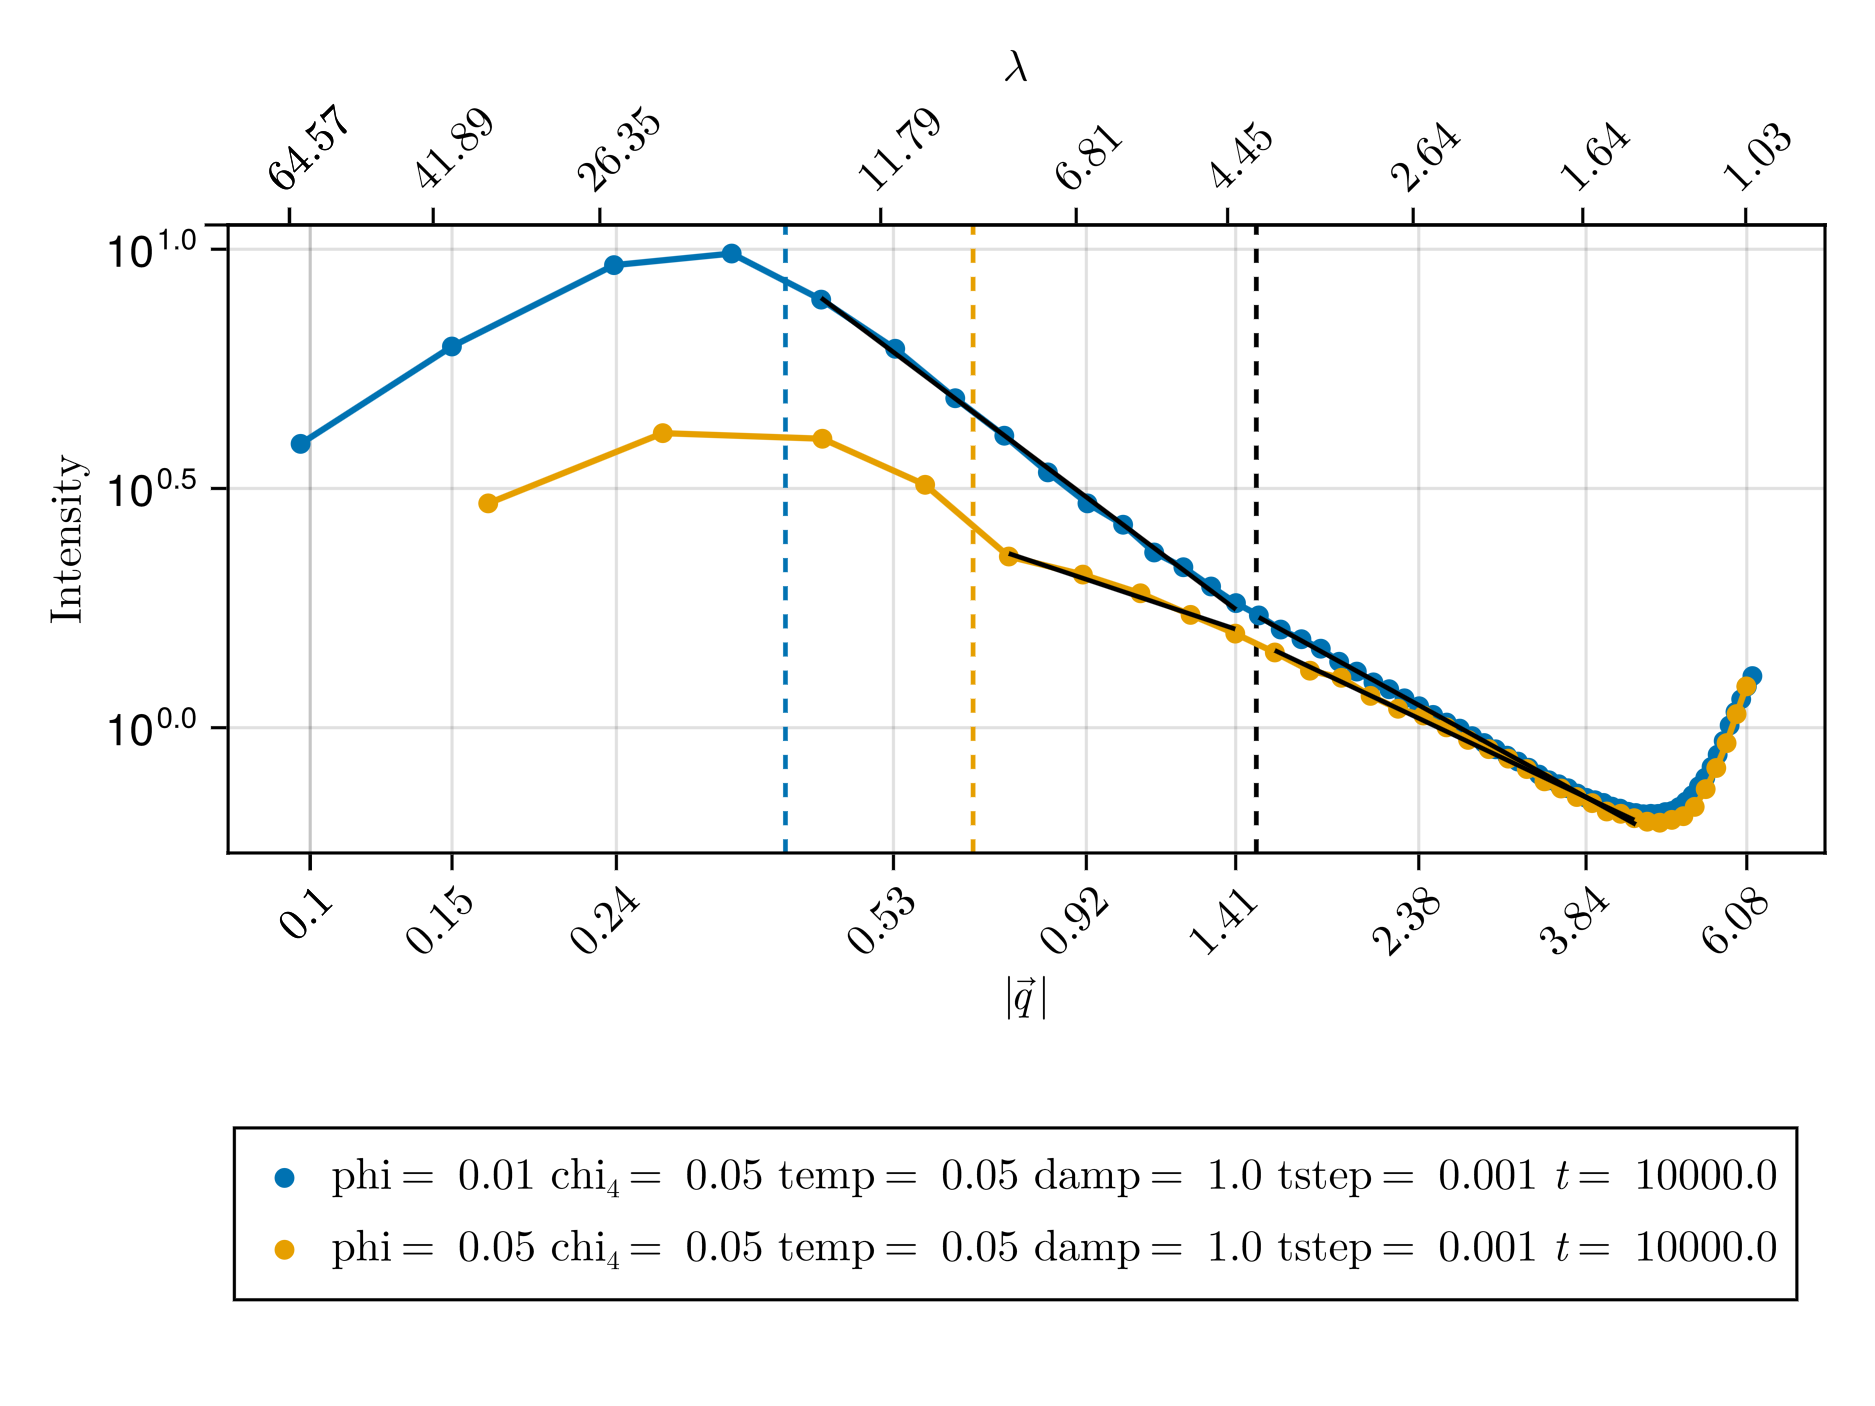
\includegraphics[width=\textwidth]{Figures/fig_Sq_tf_exp1.png}
    \caption{Structure factor of two systems with different packing fraction at the same time instant.}\label{fig:StructureFactor1}
\end{figure}

The result of the parameters are shown in the following table~\ref{tab:parameters_fit}.
The systems 1 and 2 are represented with blue and yellow colours repectively.
Finally, zone 1 is defined as \(\lambda_1\in\left[ 7/2\sigma_p,21/2\sigma_p \right]\) and zone two is defined as \(\lambda_2\in\left[ 21/2\sigma_p,L/4 \right]\).

\begin{table}[ht!]
    \centering
    \begin{tabular}{|c|c|c|c|}
    \hline
    System & Zone & A        & $\alpha$ \\ \hline
    1      & 1    & 0.925179 & 2.486543 \\ \hline
    2      & 1    & 0.794425 & 2.08354  \\ \hline
    1      & 2    & 1.264535 & 2.731100 \\ \hline
    2      & 2    & 0.561453 & 1.948924 \\ \hline
    \end{tabular}
    \caption{Results of the fit.}\label{tab:parameters_fit1}
\end{table}

\subsection{Discussion}

For me it is not clear the interpretation of $\alpha$.
On the other hand, it is intereset to see that the structure factor can be analyzed in three domains.

\section{Results Experiment 2}

An exponential fit,\(f(\abs{\vec{q}}) = \dfrac{A}{\abs{\vec{q}}^{\alpha}}\), is performed to the structure factor of the systems shown in the following figure~\ref{fig:StructureFactor}.

\begin{figure}[ht!]
    \centering
%    \includegraphics[width=\textwidth]{Figures/fig_Sq_tf_exp2.png}
    \caption{Structure factor of two systems with different packing fraction at the same time instant.}\label{fig:StructureFactor2}
\end{figure}

The result of the parameters are shown in the following table~\ref{tab:parameters_fit}.

\begin{table}[ht!]
    \centering
    \begin{tabular}{|c|c|c|c|}
    \hline
    System & Zone & A        & $\alpha$ \\ \hline
    1      & 1    & 0.925179 & 2.486543 \\ \hline
    2      & 1    & 0.794425 & 2.08354  \\ \hline
    1      & 2    & 1.264535 & 2.731100 \\ \hline
    2      & 2    & 0.561453 & 1.948924 \\ \hline
    \end{tabular}
    \caption{Results of the fit.}\label{tab:parameters_fit2}
\end{table}

\subsection{Discussion}

For me it is not clear the interpretation of $\alpha$.
On the other hand, it is intereset to see that the structure factor can be analyzed in three domains.



\section{Characteristic distances in the system and the domains for the fit}
The distance range for the pair-wise interaction is defined by the distance at minimum energy, to the cutoff, \(r_{b}\in[\sigma_p,3/2\sigma_p]\).
Then, considering that the center of all particles, central and patch, lies on the same line the distances between the center of the central particles is given by \(r_{\mathrm{int}}=2\sigma_p+r_b\).
If we evaluate $r_b$ at the limits, the interaction distance is \(r_{\mathrm{int}}\in[1.2,1.4]\).
Finally, if we increase the amount of patchy particles in pair-wise interaction, the distance between central particles is given by
\begin{gather*}
        d_{\mathrm{int}} = \left(N-1\right)\left(2\sigma_p + r_b\right).
\end{gather*}

\subsection{Zone definition of Experiment 1}

The result fo this analysis is used to defined the region at small distances.
More specifically, the lower limit of this region is set at $N=2$ and $r_b=3/2\sigma_p$ and the upper limit is set to $N=4$ and $r_b=3/2\sigma_p$.
Leading to the following spatial domain,
\begin{gather*}
    \lambda_1\in\left[ 7/2\sigma_p,21/2\sigma_p \right].
\end{gather*}
Then, we define a second spatial domain, which it's upper limit is set the order of magnitud of the total length of the simulation box, as follows,
\begin{gather*}
    \lambda_2\in\left[ 21/2\sigma_p,L/4 \right].
\end{gather*}

\subsection{Zone definition of Experiment 2}



\end{document}
